\documentclass{standalone}
\usepackage{tikz}
\begin{document}
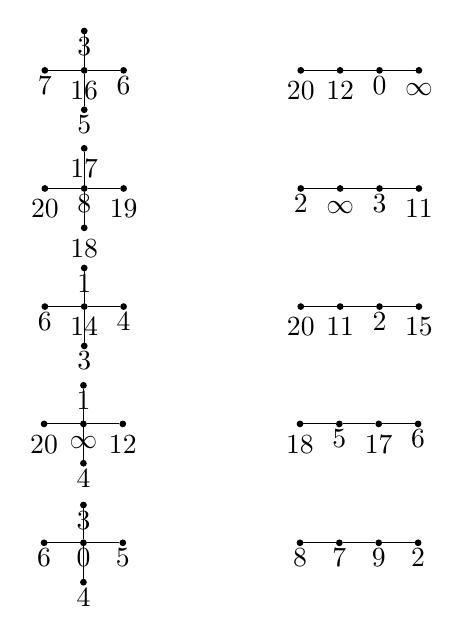
\begin{tikzpicture}[every node/.style={draw, circle, fill=black, minimum size=2pt, inner sep=0pt}]
\node[fill=black, label=below:{\color{black}$7$}] (G1N7) at (4.00,7.00) {};
\node[fill=black, label=below:{\color{black}$16$}] (G1N16) at (4.50,7.00) {};
\node[fill=black, label=below:{\color{black}$6$}] (G1N6) at (5.00,7.00) {};
\node[fill=black, label=below:{\color{black}$5$}] (G1N5) at (4.50,6.50) {};
\node[fill=black, label=below:{\color{black}$3$}] (G1N3) at (4.50,7.50) {};
\node[fill=black, label=below:{\color{black}$20$}] (G1N20) at (7.25,7.00) {};
\node[fill=black, label=below:{\color{black}$12$}] (G1N12) at (7.75,7.00) {};
\node[fill=black, label=below:{\color{black}$0$}] (G1N0) at (8.25,7.00) {};
\node[fill=black, label=below:{\color{black}$\infty$}] (G1Ninf) at (8.75,7.00) {};
\draw (G1N16) -- (G1N7);
\draw (G1N16) -- (G1N6);
\draw (G1N16) -- (G1N5);
\draw (G1N16) -- (G1N3);
\draw (G1Ninf) -- (G1N0);
\draw (G1N0) -- (G1N12);
\draw (G1N12) -- (G1N20);
\node[fill=black, label=below:{\color{black}$20$}] (G2N20) at (4.00,5.50) {};
\node[fill=black, label=below:{\color{black}$8$}] (G2N8) at (4.50,5.50) {};
\node[fill=black, label=below:{\color{black}$19$}] (G2N19) at (5.00,5.50) {};
\node[fill=black, label=below:{\color{black}$18$}] (G2N18) at (4.50,5.00) {};
\node[fill=black, label=below:{\color{black}$17$}] (G2N17) at (4.50,6.01) {};
\node[fill=black, label=below:{\color{black}$2$}] (G2N2) at (7.25,5.50) {};
\node[fill=black, label=below:{\color{black}$\infty$}] (G2Ninf) at (7.75,5.50) {};
\node[fill=black, label=below:{\color{black}$3$}] (G2N3) at (8.25,5.50) {};
\node[fill=black, label=below:{\color{black}$11$}] (G2N11) at (8.75,5.50) {};
\draw (G2N8) -- (G2N20);
\draw (G2N8) -- (G2N19);
\draw (G2N8) -- (G2N18);
\draw (G2N8) -- (G2N17);
\draw (G2N2) -- (G2Ninf);
\draw (G2Ninf) -- (G2N3);
\draw (G2N3) -- (G2N11);
\node[fill=black, label=below:{\color{black}$6$}] (G3N6) at (4.00,4.00) {};
\node[fill=black, label=below:{\color{black}$14$}] (G3N14) at (4.50,4.00) {};
\node[fill=black, label=below:{\color{black}$4$}] (G3N4) at (5.00,4.00) {};
\node[fill=black, label=below:{\color{black}$3$}] (G3N3) at (4.50,3.50) {};
\node[fill=black, label=below:{\color{black}$1$}] (G3N1) at (4.50,4.49) {};
\node[fill=black, label=below:{\color{black}$20$}] (G3N20) at (7.25,4.00) {};
\node[fill=black, label=below:{\color{black}$11$}] (G3N11) at (7.75,4.00) {};
\node[fill=black, label=below:{\color{black}$2$}] (G3N2) at (8.25,4.00) {};
\node[fill=black, label=below:{\color{black}$15$}] (G3N15) at (8.75,4.00) {};
\draw (G3N14) -- (G3N6);
\draw (G3N14) -- (G3N4);
\draw (G3N14) -- (G3N3);
\draw (G3N14) -- (G3N1);
\draw (G3N20) -- (G3N11);
\draw (G3N11) -- (G3N2);
\draw (G3N2) -- (G3N15);
\node[fill=black, label=below:{\color{black}$20$}] (G4N20) at (3.99,2.51) {};
\node[fill=black, label=below:{\color{black}$\infty$}] (G4Ninf) at (4.49,2.51) {};
\node[fill=black, label=below:{\color{black}$12$}] (G4N12) at (4.99,2.51) {};
\node[fill=black, label=below:{\color{black}$4$}] (G4N4) at (4.49,2.01) {};
\node[fill=black, label=below:{\color{black}$1$}] (G4N1) at (4.49,3.00) {};
\node[fill=black, label=below:{\color{black}$18$}] (G4N18) at (7.24,2.51) {};
\node[fill=black, label=below:{\color{black}$5$}] (G4N5) at (7.74,2.51) {};
\node[fill=black, label=below:{\color{black}$17$}] (G4N17) at (8.24,2.51) {};
\node[fill=black, label=below:{\color{black}$6$}] (G4N6) at (8.74,2.51) {};
\draw (G4Ninf) -- (G4N20);
\draw (G4Ninf) -- (G4N12);
\draw (G4Ninf) -- (G4N4);
\draw (G4Ninf) -- (G4N1);
\draw (G4N18) -- (G4N5);
\draw (G4N5) -- (G4N17);
\draw (G4N17) -- (G4N6);
\node[fill=black, label=below:{\color{black}$6$}] (G5N6) at (3.99,1.00) {};
\node[fill=black, label=below:{\color{black}$0$}] (G5N0) at (4.49,1.00) {};
\node[fill=black, label=below:{\color{black}$5$}] (G5N5) at (4.99,1.00) {};
\node[fill=black, label=below:{\color{black}$4$}] (G5N4) at (4.49,0.50) {};
\node[fill=black, label=below:{\color{black}$3$}] (G5N3) at (4.49,1.48) {};
\node[fill=black, label=below:{\color{black}$8$}] (G5N8) at (7.24,1.00) {};
\node[fill=black, label=below:{\color{black}$7$}] (G5N7) at (7.74,1.00) {};
\node[fill=black, label=below:{\color{black}$9$}] (G5N9) at (8.24,1.00) {};
\node[fill=black, label=below:{\color{black}$2$}] (G5N2) at (8.74,1.00) {};
\draw (G5N0) -- (G5N6);
\draw (G5N0) -- (G5N5);
\draw (G5N0) -- (G5N4);
\draw (G5N0) -- (G5N3);
\draw (G5N2) -- (G5N9);
\draw (G5N9) -- (G5N7);
\draw (G5N7) -- (G5N8);
\end{tikzpicture}
\end{document}
